

\section{Hash-Tree Relational Algebra}
\label{sec:impl}
%
This section discusses our implementation of efficient distributed relational algebra. We employ a hybrid approach we call \emph{Hash-Tree} RA that consists of nesting B-tree key-value stores within a hash-table that can be partitioned across multiple cores or MPI nodes. Like the double-hashing approach 



\paragraph{Hybrid hash-table and b-tree} Our approach is to use an efficient key-value store, but to



\subsection{Hybrid Join}

...

\subsection{Distributed Join}
\begin{figure*}[h]
	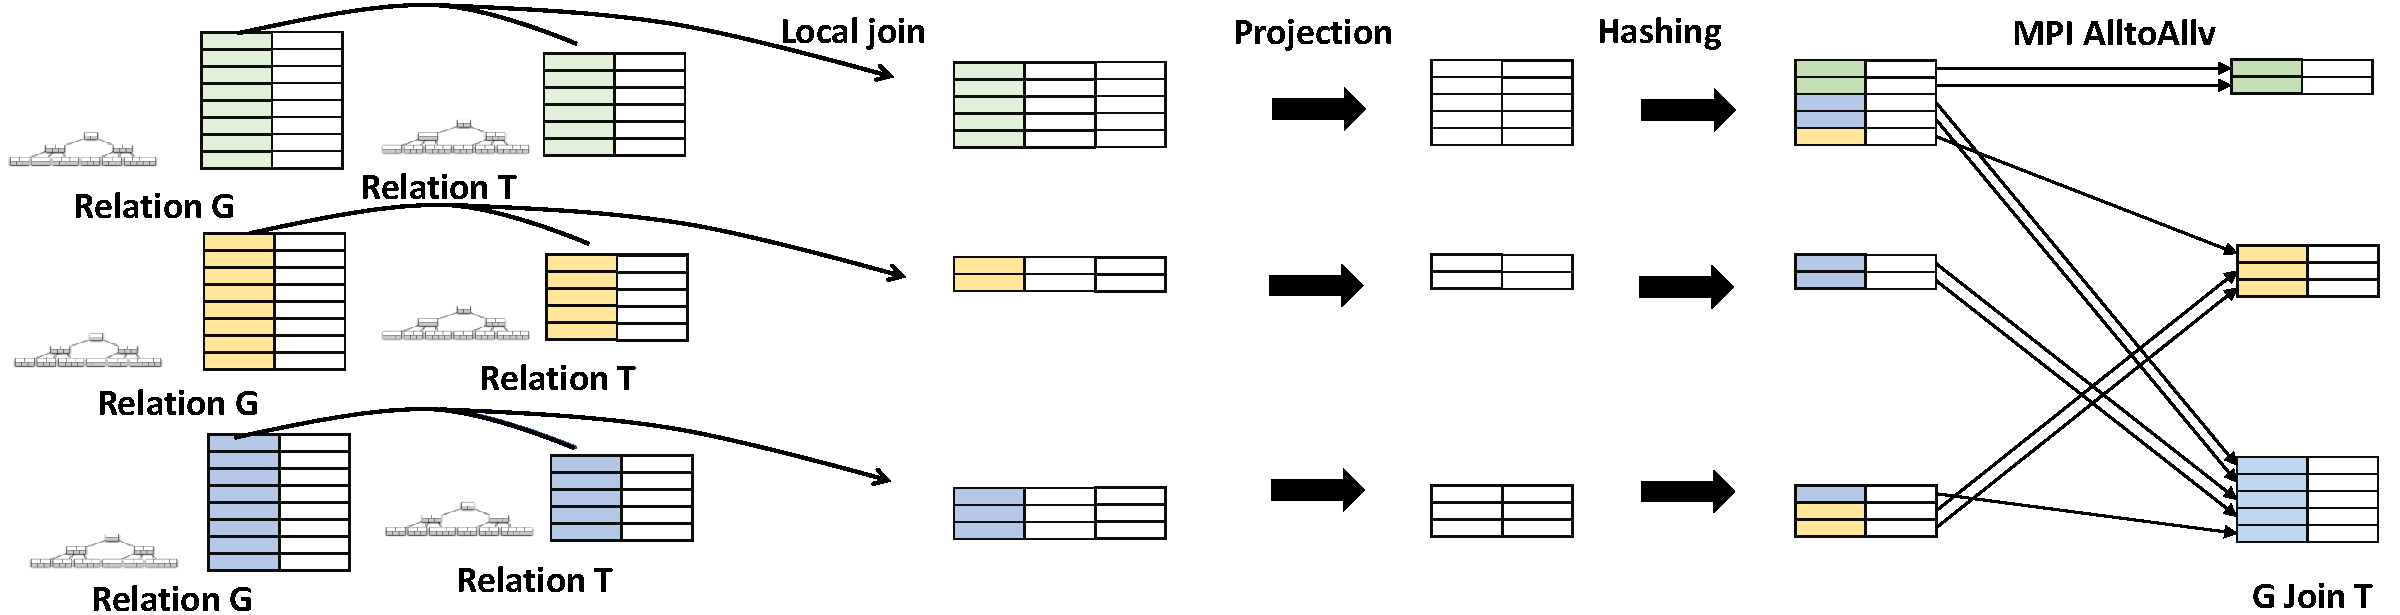
\includegraphics[width=\textwidth]{results/join_new.pdf}
	\caption{Schematic Diagram to show different phases of hash-tree join.}
	\label{fig:join}
\end{figure*}
...


\subsection{Distributed Union}
\begin{figure*}[h]
	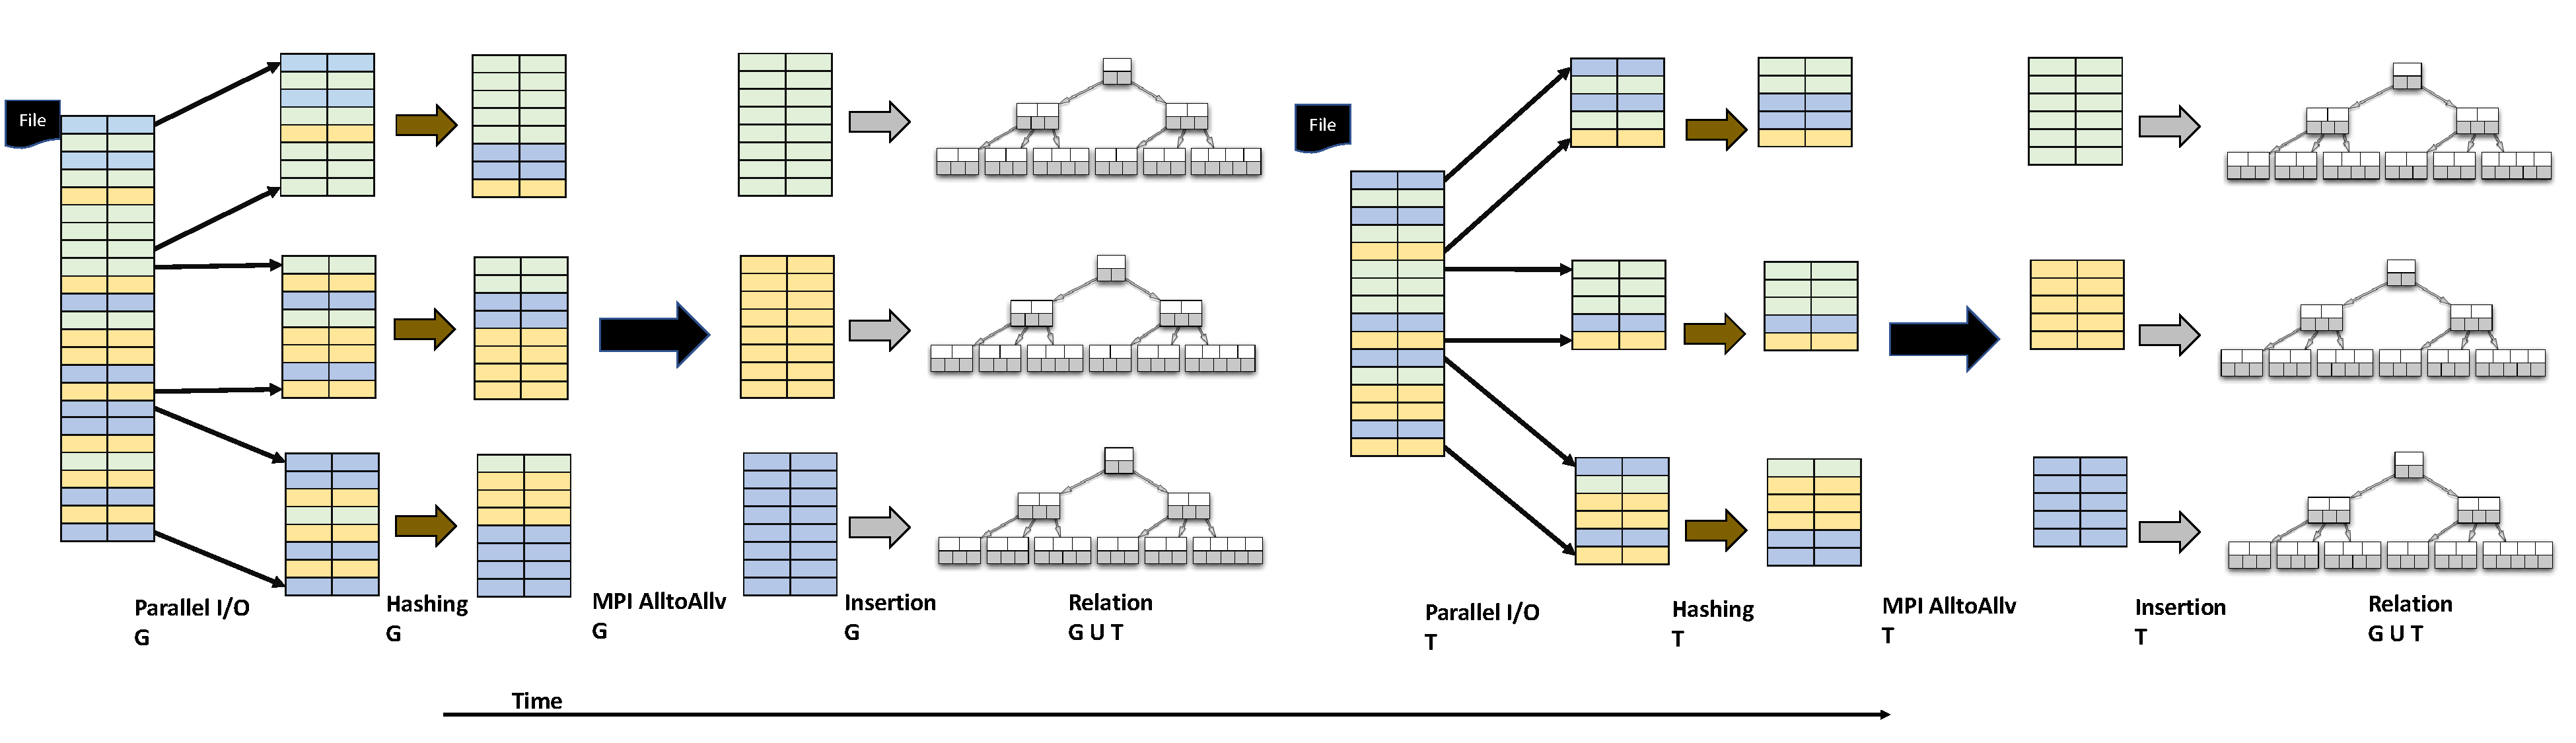
\includegraphics[width=\textwidth]{results/union_1.pdf}
	\caption{Schematic Diagram to show different phases of naive hash-tree union.}
	\label{fig:union_1}
\end{figure*}


We present two algorithms for distributed unions, buffered-hash-tree union and naive hash-tree union. As the name suggests buffered-hash-tree union buffers data across all sets that needs to be unioned before performing any communication or insertion related task. Buffered implementation has an extra memory overhead as opposed to the naive implementation where all graphs that needs to be unioned are processed one at a time.

While performing union of $n$ graphs, naive-hash-tree union involves $n$ epochs of communication and computation (one for every graph) as opposed to buffered-hash-tree union that uses buffering to limit the number of communication and computation epochs to one. 

\begin{figure}[h]
	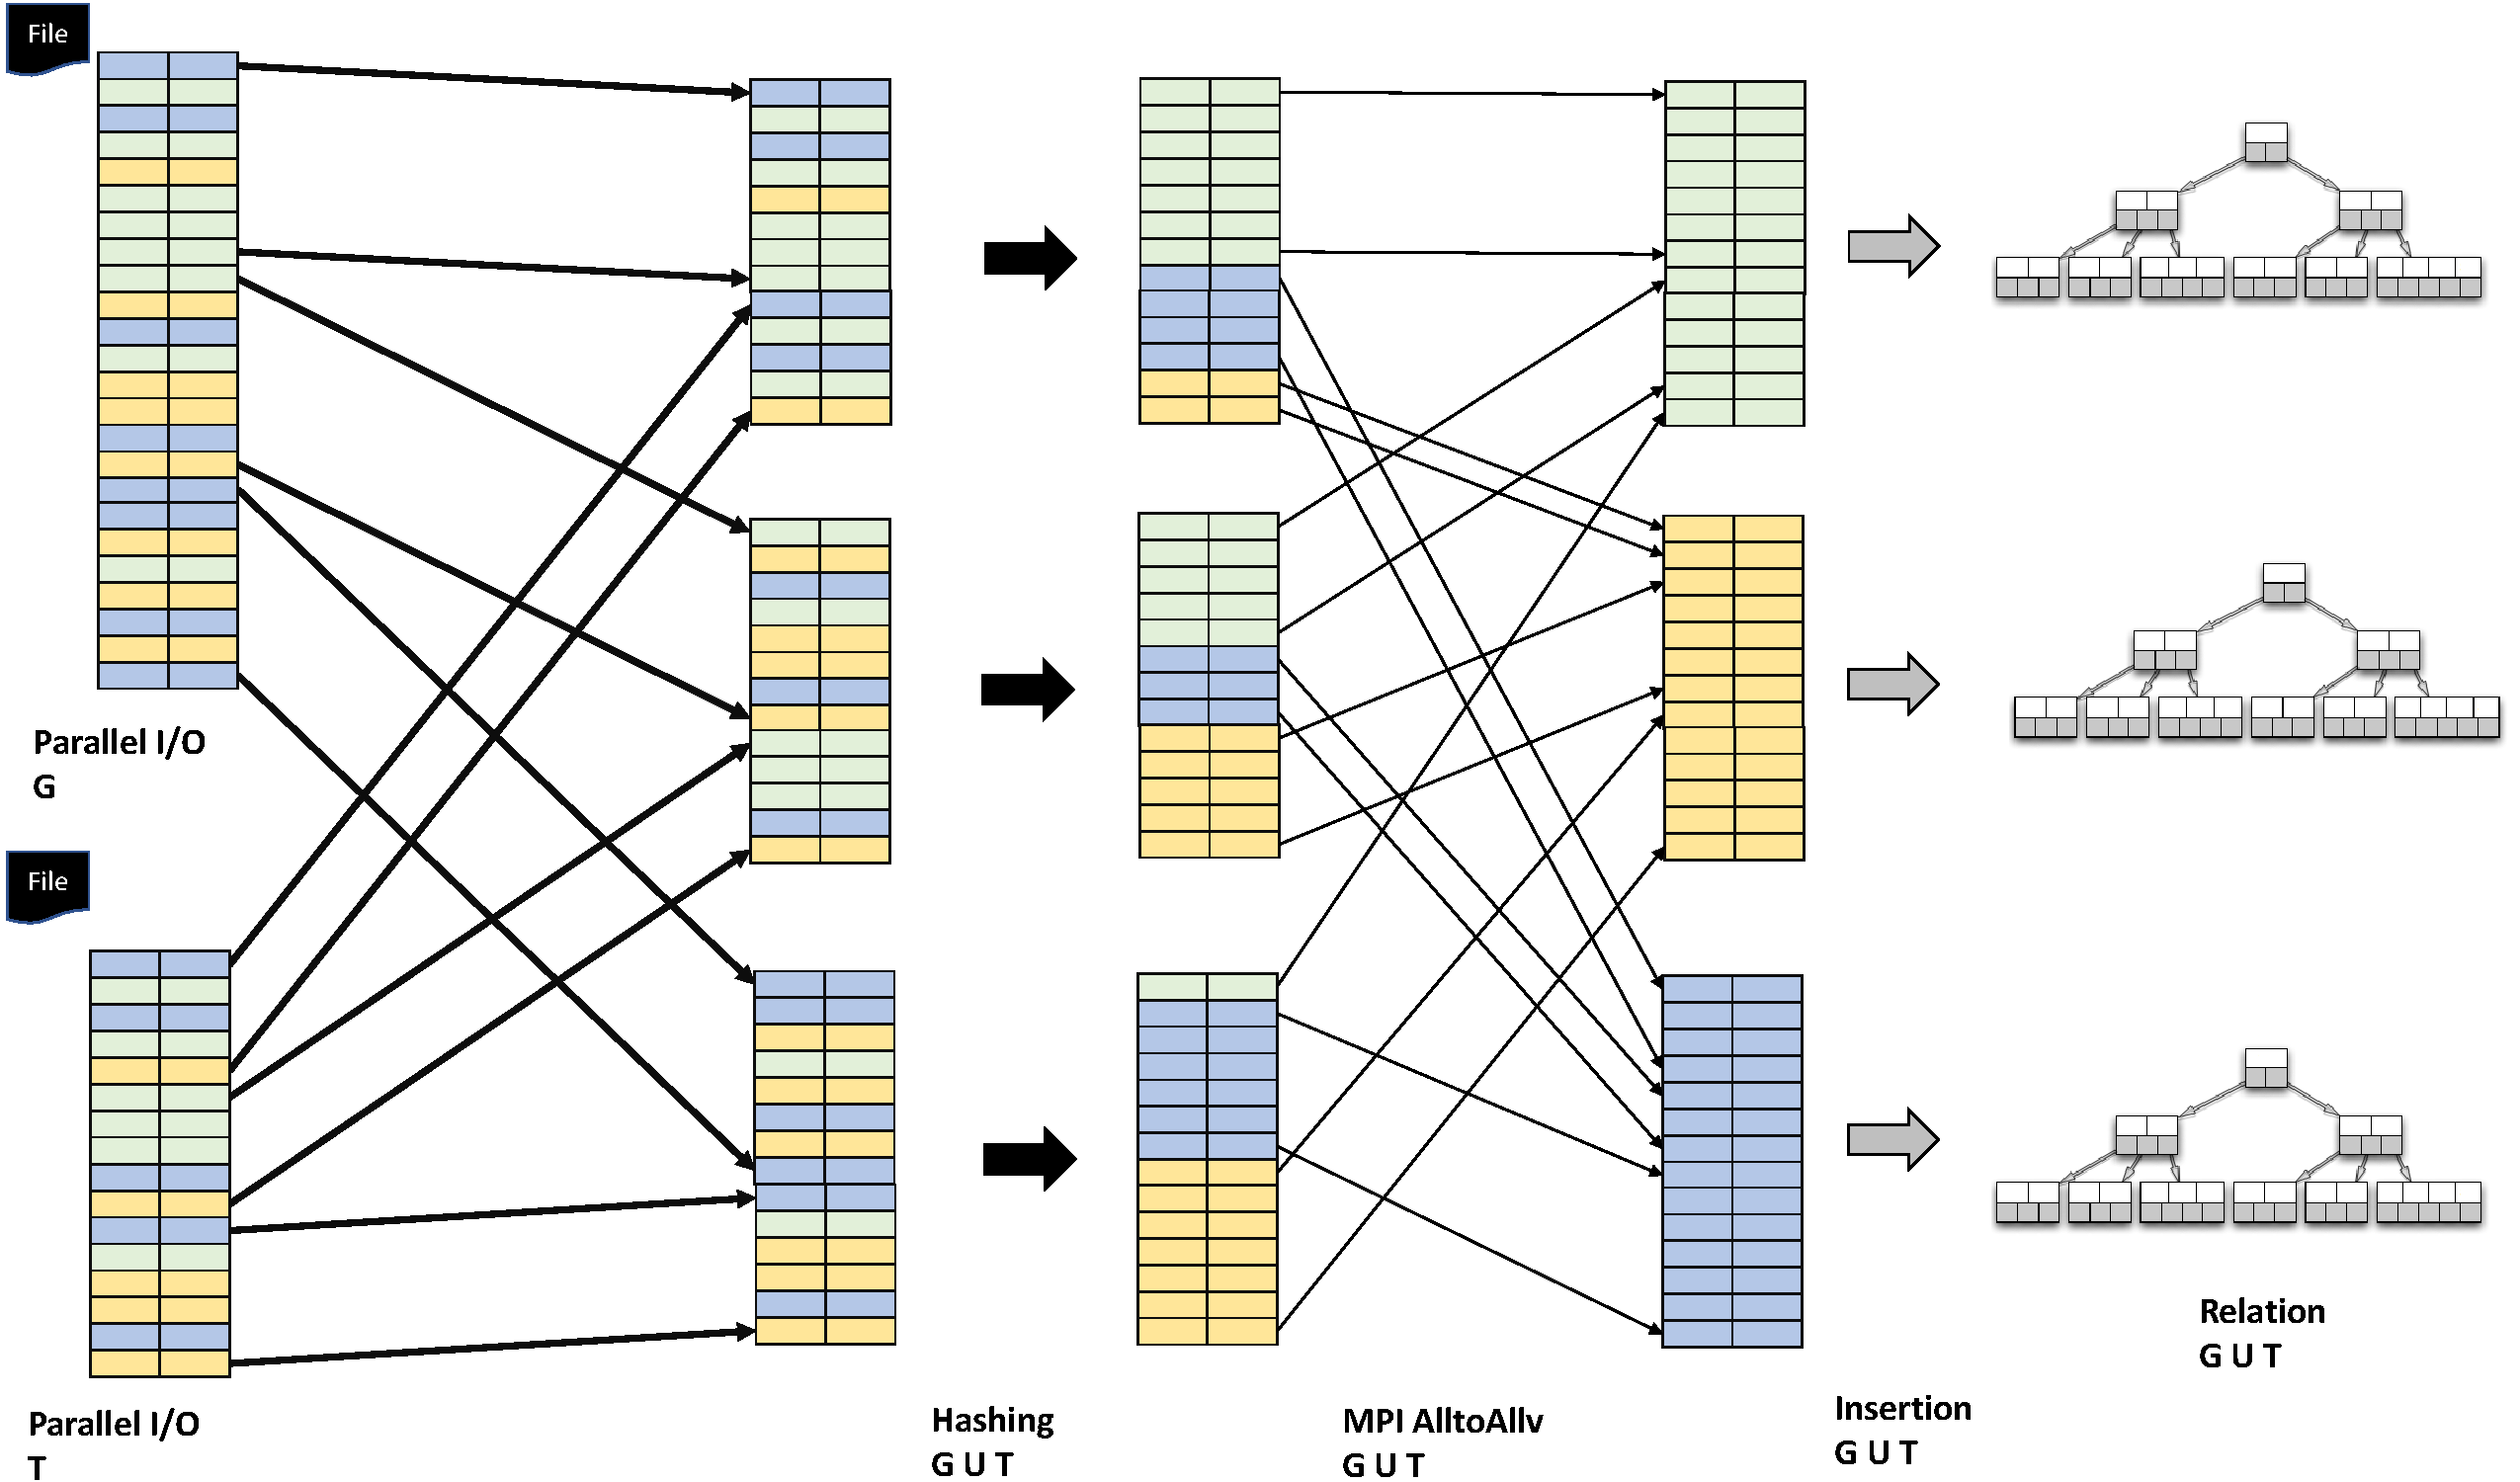
\includegraphics[width=\columnwidth]{results/union_2.pdf}
	\caption{Schematic Diagram to show different phases of buffered hash-tree union.}
	\label{fig:union_2}
\end{figure}

With the naive approach, all processes iterate through the $n$ graphs one by one.
The input graphs can be read from files stored on the disk or can be read from the memory. If the graphs are red from disk, then first phase is that of parallel I/O, where processes access disjoint regions of the file to read equal number of tuples in parallel. Once the tuples are read, every process scans through the tuples and groups them into $nprocs$ (=$hashbuckets$) packets, ready to be sent across the network.
Target process (hash-bucket) of a tuple is computed based on the hash outcome of its key. For instance, target rank of a two column tuple $(a, b)$ would be $hash(a)\%nprocs$. We also perform preliminary deduplication to eliminate duplicate tuples in the input graph. The scan step is followed actual by all to all communication phase where tuples are sent to the appropriate processes (hash buckets). Once tuples arrive at a process, they are inserted into the relation container. This step performs the important task of deduplication of tuples across the graphs. 

With buffered-hash-tree union instead of processing the graphs one after the other, we read all the graphs at once, buffer the tuples and follow it with one cumulative step of hashing, communication and insertion. Both algorithms are presented in X.